\documentclass[12pt]{article}\pagestyle{myheadings}
\usepackage{graphicx}
\usepackage{placeins}

\textwidth 7.0 truein
\oddsidemargin -0.25in   %left-hand edge
\evensidemargin -0.5 truein  %right-hand edge
\topmargin -0.85in      %top of paper to top of head, pulls whole unit
\textheight 9.5in

%Enter your last name, the portfolio problem number, and the draft number.
\title{Project 2: Flow Over a Flat Plate \\ Intermediate Numerical Analysis 1}
\author{Ian Char, Denis Kazakov, Evan Sidrow}
\date{December 1, 2015}


\usepackage{amsmath,amssymb,amsthm,amsfonts,graphicx}
%The following commands allow us to typeset theorems, propositions, definitions, etc.
\theoremstyle{plain}
\newtheorem{theorem}{Theorem}
\newtheorem{lemma}[theorem]{Lemma}
\newtheorem{corollary}[theorem]{Corollary}
\newtheorem{proposition}[theorem]{Proposition}
\newtheorem*{definition}{Definition}

\renewcommand{\qedsymbol}{\ensuremath{\blacksquare}}
\newcommand{\N}{\mathbb{N}}
\newcommand{\Z}{\mathbb{Z}}
\newcommand{\Q}{\mathbb{Q}}
\newcommand{\R}{\mathbb{R}}
\newcommand{\C}{\mathbb{C}} 

\begin{document}
\maketitle
\section{Overview}

\subsection{Introduction}

In this project, we consider a scenario where an infinitely tall mass of fluid with initial temperature $T_{\infty}$ and free stream horizontal velocity $U_{\infty}$ passes over a heated, metal plate of temperature $T_w$ ($T_w > T_{\infty}$). As a result, there are two aspects of the scenario that must be modeled: how the plate affects the velocity of the fluid, $\bar{v}(x,y) = u(x,y) \hat{i} + v(x,y) \hat{j}$, and how the plate affects the temperature of the fluid, $T(x,y)$.\vspace{5mm}

When observing the velocity of the fluid we note that as the fluid flows over the plate, it encounters friction that slows down the bottom layer of the fluid. This in turn slows down the layer on top of it, and so on. The result of this interaction is that for small values of $y, u(x, y) < U_{\infty}$ (if the value for $x$ puts the fluid past the leading edge of the plate). Additionally, $u(x, y) \rightarrow U_{\infty}$ again as $y$ becomes very large. The point at which this happens is called the momentum boundary layer and will be referred to as $\delta_m$. Lastly, it is important to note that since there is no build up of fluid there must be an induced vertical velocity in order to make the fluid flowing into a given region equal the fluid flowing out. \vspace{5mm}

The temperature of the fluid will be affected in a similar fashion. However, since $T_{w}$ is relatively hot compared to the initial temperature of the fluid, it will cause $T(x,y)$ to increase rather than decrease. In other words, when the fluid first starts to flow over the plate, the bottom layer of the fluid heats up to equal the temperature of the plate. Then, as the fluid continues to flow over the plate, the bottom layer heats up the next layer of the fluid, which heats up the next layer, and so on. Like before, we define the point at which $T(x,y) \rightarrow T_{\infty}$ to be the thermal boundary layer, and the $y$ value of this is represented as $\delta_t$ for a specific value of $x$. In this report, we analyze this system numerically in order to precisely measure it.

\section{Physical Equations}
\subsection{Transforming Three PDE's into Two ODE's}
We obtain the following equations from the laws of physics. Specifically, we obtain $(\ref{eq:massConservation})$ from Conservation of Mass,$(\ref{eq:momentumConservation})$ from Conservation of Momentum, and $(\ref{eq:energyConservation})$ from Conservation of Energy.

\begin{equation}\label{eq:massConservation}
u_x + v_y = 0
\end{equation}

where $u_x$ is the $x$ derivative of horizontal velocity and corresponds to mass flux in the $x$ direction. Likewise, $v_y$ is the $y$ derivative of vertical velocity and corresponds to mass flux in the $y$ direction.

\begin{equation}\label{eq:momentumConservation}
uu_x + vu_y = \nu u_{yy} 
\end{equation}

where $\nu$ is the kinematic viscosity of the fluid.

\begin{equation}\label{eq:energyConservation}
uT_x + vT_y = \alpha T_{yy}
\end{equation}

where $\alpha$ is the thermal diffusivity of the fluid.
\vspace{5mm}

In order to simplify the problem, we make the following transformations:\\
\begin{equation}\label{eq:u}
u = U_{\infty}F'(\eta)
\end{equation}

\begin{equation}\label{eq:v}
v = \frac{1}{2} \sqrt{\frac{\nu U_{\infty}}{x}}[\eta F'(\eta) - F(\eta)]
\end{equation}

\begin{equation}\label{eq:G}
G(\eta, Pr) = \frac{T-T_{\infty}}{T_w - T_{\infty}}
\end{equation} 

Here $Pr$ is the Prandtl number, which relates the kinematic viscosity, $\nu$, with the thermal diffusivity, $\alpha$:

{\[Pr = \frac{\nu}{\alpha} \]}

In addition, we introduce the similarity variable $\eta$, which is defined as: \\

\begin{equation}\label{eq:eta}
\eta = \frac{y}{\sqrt{\frac{\nu x}{U_{\infty}}}}
\end{equation}

After plugging in these values into the PDE's above, we obtain the following system of 2 ODE's:
\begin{equation}\label{eq:FPDE}
F''' + \frac{1}{2} FF'' = 0  
\end{equation}
\begin{equation}\label{eq:GPDE}
G'' + \frac{Pr}{2} FG' = 0 
\end{equation}



Here $F'(\eta)$ is a measure of the speed in the $x$ direction of the fluid as a proportion of free-stream conditions. In addition, $G(\eta)$ is a measure of how close the temperature of the fluid is to the temperature of the plate. To give perspective of what a particular value $\eta$ means, consider the following: at any given value of $\eta$, say $\eta_{0}$, the fluid exists along the curve:

{\[ \eta_{0} = \frac{y}{\sqrt{\frac{\nu x}{U_{\infty}}}} \]} or

\begin{equation}\label{eq:level}
 y = \frac{\eta_{0}}{\sqrt{\frac{\nu x}{U_{\infty}}}} 
\end{equation}

Therefore, we can say that on the curve described by $(\ref{eq:level})$, the values of both F and G are constant, meaning that along this curve both the temperature and velocity of the fluid in the $x$ direction are constant. Therefore, any sort of boundary layers in this problem will occur at a specific value of $\eta$.

\subsection{Finding Initial Conditions of the PDE and ODE}

Before commenting on boundary conditions, it is useful to think about what $\eta$ is doing as $x$ or $y$ approach 0 or $\infty$.

Since $x$ is in the denominator of $\eta$, $x \rightarrow 0$ means that $\eta \rightarrow \infty$, but if $x \rightarrow \infty$, then $\eta \rightarrow 0$.

Since $y$ is in the numerator of $\eta$, $y \rightarrow 0$ means that $\eta \rightarrow 0$, and if $y \rightarrow \infty$, then $\eta \rightarrow \infty$.


\vspace{5mm}
Keeping this in mind, the boundary conditions of the problem are the following: \vspace{5mm}

\begin{enumerate}
\item At the leading edge of the plate the fluid has yet to be affected by the plate. As a result, the fluid by definition has temperature $T_{\infty}$, $x$ velocity $u_{\infty}$, and $y$ velocity 0 at this point.
\begin{equation}\label{eq:leadingEdge}
T(0,y) = T_{\infty}   \,\,\,\,\,  u(0,y) = U_{\infty}    \,\,\,\,\,   v(0,y) = 0 
\end{equation}

when relating these values to the non-dimensionalized ODE, we see that all of these equations correspond to $\eta \rightarrow \infty$, since $x$ = 0. Plugging in these values in to the non-dimensionalized ODE, we get:

\begin{equation}
G(\infty) = 0  \,\,\,\,\,  U_{\infty} = U_{\infty} F'(\infty) \,\,\,\,\, 
\end{equation}
\begin{equation}
G(\infty) = 0  \,\,\,\,\,   F'(\infty) = 1 \,\,\,\,\, 
\end{equation}

Note that we are ignoring the equation $v(0,y) = 0$, as plugging this value in to the non-dimensionalized ODE results in finding that $F(\infty) \rightarrow \infty$, which is consistent with $F'(\infty) = 1$.

\item Along the base of the plate, since velocity and temperature close to the plate must match that of the plate, the fluid remains stationary next to the plate and heats up to match $T_{w}$.
\begin{equation}\label{eq:alongEdge}
T(x,0) = T_{w}   \,\,\,\,\,  u(x,0) = 0    \,\,\,\,\,   v(x,0) = 0
\end{equation}

Note that when y = 0, $\eta$ = 0. plugging in these values to the non-dimensionalized ODE, we get:

\[G(0) = \frac{T_{w}-T_{\infty}}{T_{w}-T_{\infty}} = 1   \,\,\,\,\,  0 = U_{\infty} F'(0)    \,\,\,\,\,    0 = \frac{1}{2} \sqrt{\frac{\nu U_{\infty}}{x}}[0 * F'(0) - F(0)]\]
\begin{equation}
G(0) = 1   \,\,\,\,\,  F'(0) = 0  \,\,\,\,\,  F(0) = 0
\end{equation}


\item When fluid is far enough from the plate, it is no longer affected by it. Therefore, it takes on the same conditions as free flow values (at least in x velocity and temperature):

\begin{equation}\label{eq:farFromPlate}
T(x,\infty) = T_{\infty}   \,\,\,\,\,  u(x,\infty) = U_{\infty} 
\end{equation}

Note that when $y \rightarrow \infty$ , $\eta \rightarrow \infty$. Plugging in these values to the non-dimensionalized ODE, we get:

\[
G(\infty) = \frac{T_{\infty}-T_{\infty}}{T_{w}-T_{\infty}} = 0   \,\,\,\,\,  U_{\infty} = U_{\infty} F'(\infty)    \,\,\,\,\, 
\]

\begin{equation}
G(\infty) = 0   \,\,\,\,\,  F'(\infty) = 1   \,\,\,\,\, 
\end{equation}

\end{enumerate}

In summary, the boundary conditions for the non-dimensionalized ODE are:

\begin{eqnarray*} 
F(0) = 0 \\
F'(0) = 0 \\ 
F'(\infty) = 1 \\
G(0) = 1 \\
G(\infty) = 0 \\
\end{eqnarray*}

\section{Modeling the Fluid}
\subsection{Integration of ODEs}
We first consider the system of ODEs consisting of $(\ref{eq:FPDE})$ and $(\ref{eq:GPDE})$ where $Pr = 5$. Although there is no way to find a closed form solution for $F(\eta)$ and $G(\eta)$, the behavior of the solution can be modeled through numerical integration. To integrate the ODEs, 4th order Runge-Kutta can be used with a step size of $\Delta \eta= 0.1$. Since $(\ref{eq:FPDE})$ is independent of $(\ref{eq:GPDE})$, we can start by finding a solution to $F(\eta)$ and then solve for $G(\eta)$. One significant obstacle that bars us from simply using Runge-Kutta to find the solutions to the problem is that we lack initial conditions for $F''(\eta)$ and $G'(\eta)$. However, we are given that $F'(\eta) \rightarrow 1$ and $G(\eta) \rightarrow 0$ as $\eta \rightarrow \infty$. Using this information we can use a shooting technique where we guess initial values of $F''(\eta)$ and $G'(\eta)$ until they satisfy the aforementioned boundary conditions to five digits. The first 10 and last 10 iterations of the integration are listed in Table 1 where the integration goes from $\eta = 0$ to $\eta = 15$. 

\begin{table}[ht!]
\centering
\begin{tabular} {| l | l | l | l | l | l |}
\hline
$\eta$ & $F(\eta)$ & $F'(\eta)$ & $F''(\eta)$ & $G(\eta)$ & $G'(\eta)$ \\
\hline
0.0 & 0.0 & 0.0 & 0.3320573 & 1.0 & -0.5766881 \\
0.1 & 0.0016603 & 0.0332055 & 0.3320481 & 0.9423332 & -0.5766083 \\
0.2 & 0.006641 & 0.0664078 & 0.3319838 & 0.8846943 & -0.5760501 \\
0.3 & 0.0149415 & 0.0995986 & 0.3318093 & 0.827155 & -0.5745379 \\
0.4 & 0.0265599 & 0.1327641 & 0.3314698 & 0.7698341 & -0.5716046 \\
0.5 & 0.0414928 & 0.1658852 & 0.3309109 & 0.7128964 & -0.566802 \\
0.6 & 0.0597347 & 0.1989372 & 0.3300791 & 0.65655 & -0.5597138 \\
0.7 & 0.081277 & 0.2318902 & 0.328922 & 0.6010422 & -0.5499722 \\
0.8 & 0.1061082 & 0.2647091 & 0.3273892 & 0.5466541 & -0.5372766 \\
0.9 & 0.134213 & 0.2973539 & 0.3254326 & 0.4936927 & -0.5214123 \\
... & ... & ... & ... & ... & ... \\
14.1 & 12.3792112 & 0.9999999 & 0.0 & 1e-06 & -0.0 \\
14.2 & 12.4792112 & 0.9999999 & 0.0 & 1e-06 & -0.0 \\
14.3 & 12.5792112 & 0.9999999 & 0.0 & 1e-06 & -0.0 \\
14.4 & 12.6792112 & 0.9999999 & 0.0 & 1e-06 & -0.0 \\
14.5 & 12.7792112 & 0.9999999 & 0.0 & 1e-06 & -0.0 \\
14.6 & 12.8792111 & 0.9999999 & 0.0 & 1e-06 & -0.0 \\
14.7 & 12.9792111 & 0.9999999 & 0.0 & 1e-06 & -0.0 \\
14.8 & 13.0792111 & 0.9999999 & 0.0 & 1e-06 & -0.0 \\
14.9 & 13.1792111 & 0.9999999 & 0.0 & 1e-06 & -0.0 \\
15.0 & 13.2792111 & 0.9999999 & 0.0 & 1e-06 & -0.0 \\

\hline
\end{tabular}
\caption{Interpolated values of $\eta_{m}$ and $\eta_{t}$}
\end{table}

\pagebreak

\subsection{Analysis of Velocity}
In order to analyze velocity, we recall $(\ref{eq:u})$ and $(\ref{eq:v})$. For these equations, we know that $F'(\eta)$ is a measure of horizontal velocity and that $\frac{1}{2}[\eta F'(\eta) - F(\eta)]$ is a measure of vertical velocity. In particular,

\begin{equation*}
F'(\eta) = \frac{u}{U_{\infty}}
\end{equation*}

\begin{equation*}
\frac{1}{2}(\eta F'(\eta) - F(\eta)) = \frac{v}{U_{\infty}} \sqrt{\frac{x}{L}} \sqrt{Re}
\end{equation*}

Where Re is the Reynold's number, which is related to the turbulence of the flow of the fluid. Re is proportional to the free flow velocity of fluid ($U_{\infty}$), the length of the plate ($L$), and the inverse of the kinetic viscosity of the fluid ($\frac{1}{\nu}$).

With respect to the horizontal velocity, we know that once $u$ reaches the value of $U_{\infty}$, the ratio of $\frac{u}{U_{\infty}}$ will be 1. Therefore, we know that the value of $\eta$ (which we will define as $\eta_{m}$) for which $F'(\eta_{m}) = 1$ is the value when the horizontal velocity returns to its free stream velocity. In other words, $\eta_{m}$ is the proportion of $y$ and $x$ that describes $\delta_{m}$. This way, $\eta_{m}$ gives us an equation for the thickness of momentum boundary layer, which we can derive from $(\ref{eq:eta})$:\\
\begin{equation}\label{eq:momentumBoundary}
y = \eta_{m} \sqrt{\frac{\nu x}{U_{\infty}}}
\end{equation}

While the true value of $\eta_{m}$ is when $F'(\eta) \rightarrow 1$, we choose to use the condition of when $F'(\eta)$ equals a value slightly smaller than $1$ since $F'(\eta)$. Therefore, for this project we assume $\eta_{m}$ to be the value at which $F'(\eta) = 0.97$ (note that the exact $\eta_{m}$ value will be interpolated later in the paper). In order to visualize this process, we can plot $\frac{1}{2}(\eta F'(\eta) - F(\eta))$ (proportional to $v$), $F'(\eta)$ (proportional to $u$), and $\eta_{m}$ on the same graph (Figure $\ref{fig:velocities}$).



\begin{figure}[ht!]
\centering
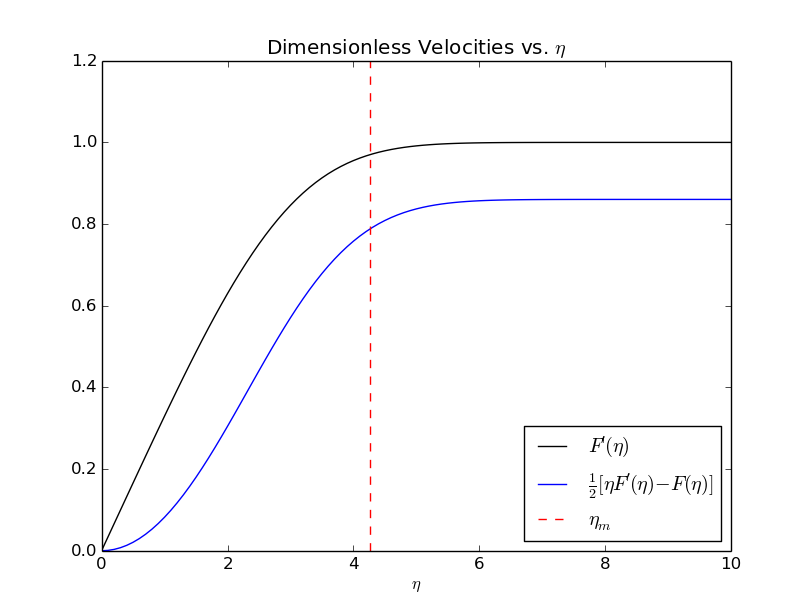
\includegraphics[scale=0.75]{dimvel.png}
\caption{A plot of the dimensionless velocities for $u(x,y)$ and $v(x,y)$ along with the $\eta_{m}$ representing the momentum boundary layer.}
\label{fig:velocities}
\end{figure}

There are several important physical implications that can be taken away from Figure $\ref{fig:velocities}$. First of all, past $\eta_{m}$ both $F'(\eta)$ and $\frac{1}{2}(\eta F'(\eta) - F(\eta))$ level off. This is as expected since once the momentum boundary layer has been crossed, the horizontal velocity of the fluid should not continue increasing; it returns to what it was at free stream. Likewise, since the horizontal rate of flow onto the plate equals the horizontal rate of flow off of the plate for the fluid above the momentum boundary layer, there is no longer a need for an induced vertical velocity. As such, $v(x,y)$ stays constant.

\subsection{Analysis of Temperature}
For the temperature of the fluid we look at how $G(\eta)$ is defined in $(\ref{eq:G})$. It should be noted that unlike the velocity of the fluid, $Pr$ does have an affect on the outcome of $G(\eta)$. However, like $F'(\eta)$, we can determine information about boundary layers from the solution (specifically $\eta_{t}$, which corresponds to the thermal boundary layer). According to the definition, as $T$ approaches $T_{\infty}$, $G(\eta)$ approaches $0$. On the other hand, as $T$ approaches $T_{w}$, $G(\eta)$ approaches $1$. Because of this, the thermal boundary layer occurs where $G(\eta_{t}) \rightarrow 0$. Like before, we approximate $\eta_{t}$ to be the value of $\eta$ for when $G(\eta) = 0.03$. In Figure $\ref{fig:temps}$, $G(\eta)$ is plotted with the $Pr$ values of 0.2, 2, 5, and 10. Additionally, the black dot indicates the position at which $\eta_{t}$ occurs on each curve.

\begin{figure}[ht!]
\centering
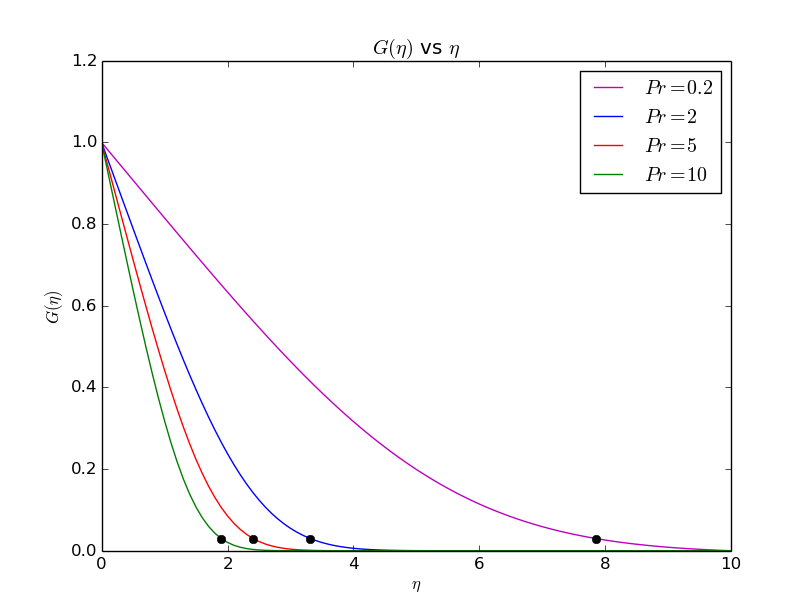
\includegraphics[scale=0.75]{Gs.png}
\caption{Values of $G(\eta)$ for different $Pr$ and marked $\eta_{t}$}
\label{fig:temps}
\end{figure}

From Figure $\ref{fig:temps}$ we are able to observe an important relation between $Pr$ and $\delta_{t}$. As $Pr$ increases, one does not have to move as far away from the plate to return to $T_{\infty}$ with respect to the momentum boundary layer. This will be discussed further in Section 3.6.

\subsection{Interpolation of $\eta_{m}$ and $\eta_{t}$}
Previously, we sought values of $\eta_{m}$ and $\eta_{t}$ such that $F'(\eta_{m}) = 0.97$ and $G(\eta_{t}) = 0.03$. However, it is improbable that $F'$ and $G$ would ever exactly equal $0.97$ and $0.03$ for values generated in Table 1. In order to get an exact $\eta_{m}$ and $\eta_{t}$, we can predict what $\eta$ should be through Newton's interpolation method.\vspace{5mm}

To do this, we pick out five neighboring points for both our desired $\eta_{m}$ and our desired $\eta_{t}$. Using these five points along with Newton's interpolation method, two fourth degree polynomials of $\eta$ are generated and used to predict their respective boundary density thickness. An important thing to note is that in generating the polynomials, $F'(\eta)$ and $G(\eta)$ take on what would be traditionally be thought of as the $x$ axis while $\eta$ serves as the $y$ axis since we want to interpolate values of $\eta$. Furthermore, although the value of $\eta_{t}$ changes when $Pr$ changes, $\eta_{m}$ stays consistent since the PDE for $F(\eta)$, $(\ref{eq:FPDE})$, does not involve $Pr$. The values of $\eta_{m}$ and $\eta_{t}$ are displayed in Table 2.


\begin{table}[ht!]
\centering
\begin{tabular} {| l | l | l | l | l | l |}
\hline
$Pr$ & $\eta_{m}$ & $\eta_{t}$ \\
\hline
0.2 & 4.26265401028 & 7.84766218463 \\
2 & 4.26265401028 & 3.31278707023 \\
5 & 4.26265401028 & 2.40632125468 \\
10 & 4.26265401028 & 1.90018392625 \\
\hline
\end{tabular}
\caption{Interpolated values of $\eta_{m}$ and $\eta_{t}$}
\end{table}

\subsection{Trends of Boundary Layers}
Now that we have values for $\eta_{m}$ and $\eta_{t}$, we can use the definition of $\eta$ to derive a relation between $x$ and $y$. \\
$$y = \frac{\eta}{\sqrt{\frac{\nu x}{U_{\infty}}}} $$
$$\frac{y\sqrt{Re}}{L} = \frac{\eta}{\sqrt{\frac{\nu x}{U_{\infty}}}} \frac{\sqrt{Re}}{L}$$

We interpret $\delta_m$ and $\delta_t$ as a difference across y dimension. Therefore, after plugging in $Re = \frac{U_{\infty}L}{\nu} $ into $\frac{\delta_m}{L}\sqrt{Re} $, we are left with: \\

$$\frac{\delta \sqrt{Re}}{L} =  \eta{\sqrt{\frac{\nu x U_{\infty} L}{U_{\infty} \nu L^2}}} = \eta \sqrt{\frac{x}{L}}$$

Therefore, we plot the following relations:
\[\delta_m \sqrt{\frac{U_{\infty}}{\nu}} = \eta_m \sqrt{x}  \,\,\,\,\,\,\,\,\,\,  \delta_t \sqrt{\frac{U_{\infty}}{\nu}} = \eta_t \sqrt{x}\]

\begin{figure}[h]
\centering
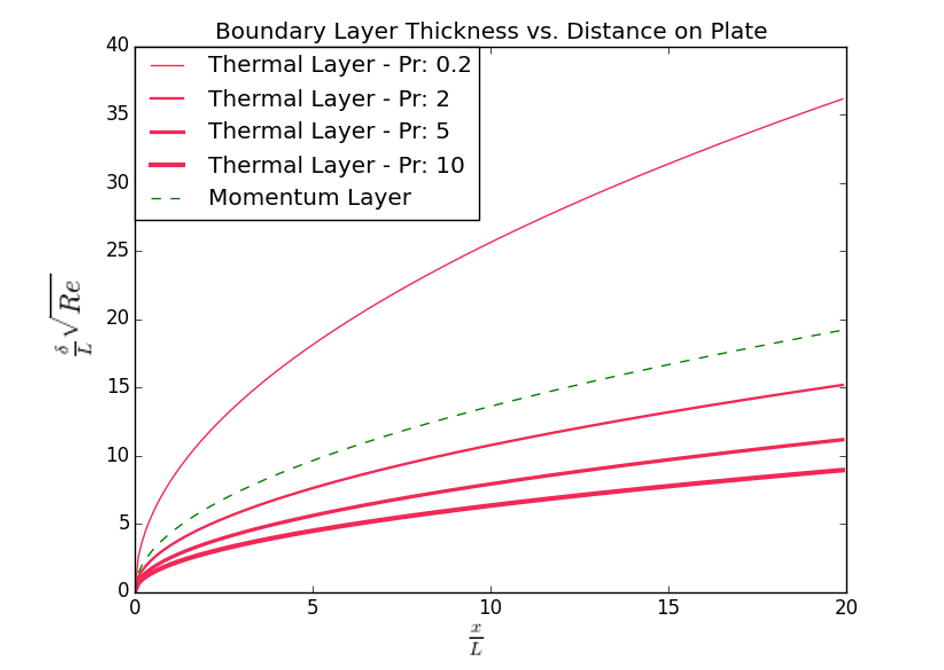
\includegraphics[scale=0.75]{part5.png}
\caption{The thickness of thermal and momentum boundary layers as a function of distance across the plate.}
\label{fig:boundaryLayers}
\end{figure}

Figure $\ref{fig:boundaryLayers}$ shows the square root nature behind the boundary layer trends. In addition to this, we can also see that as $Pr$ becomes larger, the thermal boundary layer becomes narrower. However, it can only get so narrow, and the rate at which the boundary layer narrows decreases as $Pr$ grows larger and larger.

\break

\subsection{Relation of $Pr$ and $\eta_{t}$}
As discussed in Section 3.3, $Pr$ has a direct effect on $\eta_{t}$. The higher $Pr$ is, the smaller the thermal boundary layer thickness will be. This can be seen in Figure $\ref{fig:etats}$.

\begin{figure}[ht!]
\centering
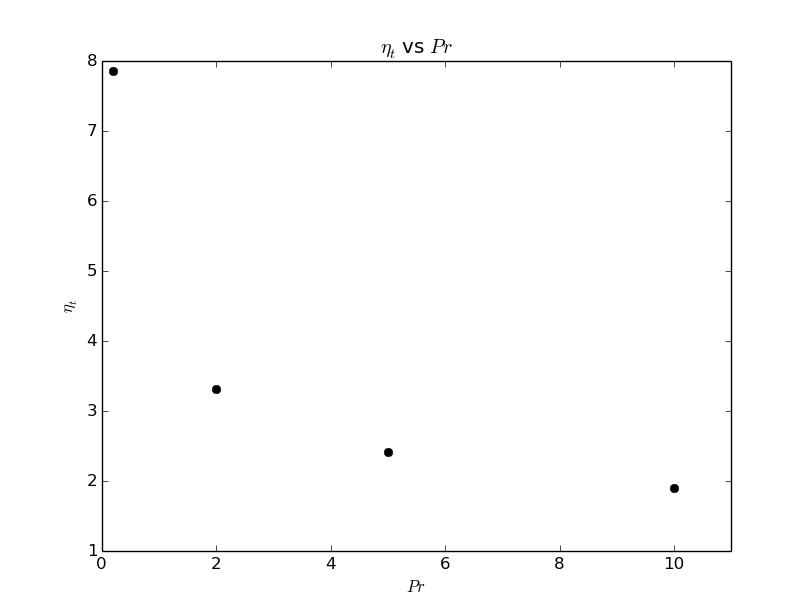
\includegraphics[scale=0.6]{part6.png}
\caption{A plot of the different thermal boundary layers with respect to $Pr$.}
\label{fig:etats}
\end{figure}

\break

This relation makes sense because $Pr$ is proportional to $\nu$ and inversely proportional to $\alpha$. If $\nu$ becomes larger (and therefore $Pr$ becomes larger), then the viscosity of the fluid is increased, increasing the momentum boundary layer. Since the thermal boundary layer is measured with respect to the momentum boundary layer, then the relative size of the thermal boundary layer will go down, decreasing $\eta_{t}$. If $\alpha$ becomes larger (and therefore Pr becomes smaller), then the thermal diffusivity of the fluid is increased and the size of the thermal boundary layer is increased, increasing $\eta_{t}$.


\section{Conclusion}
Through the numerical solutions that have been performed throughout this lab, we are able to get an insight to the physical nature behind this problem. As fluid moves over a heated plate, the bottom layer of the fluid "sticks" to the plate (velocity = 0) and heats up to match the temperature of the plate (temperature = $T_w$). Due to both heat convection and friction, these lower layers of fluid heat up and slow down the fluid above it. Using the properties of conservation of mass, conservation of momentum in the x direction, and conservation of energy, we were able to nondimensionalize the problem by introducing a similarity variable 

{\[ \eta = \frac{y}{\sqrt{\frac{\nu x}{U_{\infty}}}} \]}

. This reduced a system of PDE's to a system of ODE's which describe the speed of the fluid ($F(\eta)$) as well as the temperature ($G(\eta)$) along set values of $\eta$. This similarity variable also gives insight into the physics of the problem, as any given value of $\eta$ creates a curve of $x$ and $y$ values at which the fluid has constant the temperature and velocity in the $x$ direction.

Since this system is subject to conservation of mass, the slowing of the fluid in the $x$ direction close to the plate causes mass to accumulate, but this mass must be disposed of in order to conserve mass. The only place for the mass to go is in the positive y direction, so there is an induced fluid flow in the positive y direction which propagates upward indefinitely to $y \rightarrow \infty$.

Any given value of $\eta$ creates a curve of $x$ and $y$ values at which the fluid has constant temperature and constant velocity (in the x direction). Therefore, certain values for $\eta$ ($\eta_{t}$ and $\eta_{m}$) were used to find boundary conditions. Above these boundary conditions, the fluid essentially doesn't notice the plate, neither in its temperature nor its velocity in the x direction. Also, since $\eta$ is a function of $\nu$, changing $\nu$ does not effect the boundary momentum layer in nondimensionalized units. Therefore, the Prandatl number, $Pr = \nu / \alpha$, is used to relate the momentum boundary layer to the thermal temperature layer. If Pr is high, then the thermal diffusivity is low compared to the kinetic viscosity, so thermal energy cannot move as easily as momentum can and the thermal boundary layer is small compared to the momentum boundary layer. On the other hand, if Pr is low, the opposite is true, and the thermal boundary layer is large compared to the momentum boundary layer.

All of these conclusions are supported by the numerical methods used in the analysis done throughout this report. These numerical calculations, therefore, are vital - not only to determine precise measurements of boundary layers and induced velocities, but also to achieve a  physical understanding of the solution to the problem itself.


\end{document}